\clearpage
\section{Converting Between Degrees and Radians}
Now you'll learn how to convert between degrees and radians.

The formulas are as follows:
\begin{itemize}
    \item Radians to Degrees $rad \times \frac{180}{\pi}$.
    \item Degress to Radians $deg \times \frac{\pi}{180}$.
\end{itemize}
To understand why this works, let's look at the unit circle again.
\begin{center}
    \begin{minipage}[t]{0.35\textwidth}
        \centering
        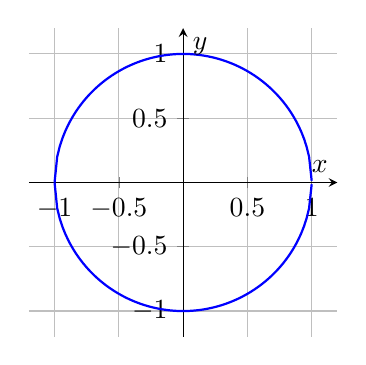
\begin{tikzpicture}[baseline=(current bounding box.north)]
            \begin{axis}[
                axis lines = middle,
                xlabel = $x$, ylabel = {$y$},
                xmin = -1.2, xmax = 1.2,
                ymin = -1.2, ymax = 1.2,
                xtick distance={0.5}, ytick distance={0.5},
                width = 5.5cm,
                height = 5.5cm,
                grid = both,
                legend pos = south east,
            ]
                \addplot[blue, thick, domain=-1:1, samples=100] {sqrt(1 - x^2)};
                \addplot[blue, thick, domain=-1:1, samples=100] {-1 * sqrt(1 - x^2)};
            \end{axis}
        \end{tikzpicture}
    \end{minipage}%    <-- % important to avoid a space
    \begin{minipage}[t]{0.64\textwidth}
        A circle has $360 \degree$. That is, if we start in the positive $x$ direction and traveled around the circle until we ended where we started, we would've traveled a full $360\degree$ around the circle. 
        \\ \\
        Knowing what we know about radians, we could also say that travling around the circle menas we did a full $2\pi$ radians around the circle.
    \end{minipage}
\end{center}
With this in mind, we can agree that $360\degree = 2\pi\,rad$. So, technically, $\frac{360}{2\pi} = 1$.

Conversely, $\frac{2\pi}{360} = 1$ also.

Simplifying both of these gives:
\begin{align*}
    \frac{360}{2\pi} = 1 &\Longrightarrow \frac{180}{\pi} = 1 \\
    \frac{2\pi}{360} = 1 &\Longrightarrow \frac{\pi}{180} = 1
\end{align*}
When converting, because the numerator is the same as the denominator, multiplying a value by this factor doesn't change it.

For example, if we had $\frac{\pi}{2}$ radians and we wanted to convert this to degrees, we'd multiply it by $\frac{180}{\pi}$.
\begin{align*}
    \frac{\pi}{2}\,rad  \cdot \frac{180}{\pi} &= \frac{180\pi}{2\pi} = 90\degree \\
\end{align*}
It's easy to forget which equation you should when converting. Here's how I remember it.
\begin{itemize}
    \item If an angle in radians is equal to that same measurement in degrees, the actual number in radians is \textit{always} smaller (i.e. $2\pi$, which is approximately $6.28$, is \textit{much} smaller than $360$). If we actually divide $\frac{\pi}{180}$, we get approximately $0.017453$, which is a really smaller number.
    
    Anything $\times$ Number less than $1$ $=$ Smaller Number.

    So, when converting from degrees to radians, we want to use $\frac{\pi}{180}$.

    \item Likewise, if an angle in radians is equal to an angle in degrees, the value in degrees is \textit{always} greater (i.e. $360$ is a lot bigger than $2\pi \approx 6.28$). If we divide $\frac{180}{\pi}$, we get approximately $57.29578$, which is pretty big.
    
    Anything $\times$ Number greater than $1$ $=$ Bigger Number.

    So, when converting from radians to degrees, we want to use $\frac{180}{\pi}$.
\end{itemize}
Let's try a few conversions together.
\begin{problem}
    Convert $45$ degrees to radians.
\end{problem}
\begin{solution}
    Since we're converting \textit{from} degrees \textit{to} radians, we need to use $\frac{\pi}{180}$.
    \begin{align*}
        45 \cdot \frac{\pi}{180} &= \frac{45\pi}{180}\\
        &= \frac{\pi}{4} && 45 \cdot 4 = 90 \cdot 2 = 180
    \end{align*}
\end{solution}
\clearpage
\begin{problem}
    Convert $\frac{\pi}{6}$ radians to degrees.
\end{problem}
\begin{solution}
    This time, we're converting \textit{from} radians \textit{to} degrees. So we need to use $\frac{180}{\pi}$.
    \begin{align*}
        \frac{\pi}{6} \cdot \frac{180}{\pi} &= \frac{180\pi}{6\pi} \\
        &= 30
    \end{align*}
\end{solution}
Let's do one last one just to make sure you're paying attention.
\begin{problem}
    Convert $1.5708$ radians to degrees.
\end{problem}
\begin{solution}
    Once again, we're converting from radians to degrees. So we must use $\frac{180}{\pi}$.
    \[
        1.5708 \cdot \frac{180}{\pi} = \frac{180(1.5708)}{\pi}
    \]
    This evaluates to roughly $90.00021\degree$. This value is almost $90\degree$. That's because $1.5708$ is approximately $\frac{\pi}{2}$, and $\frac{\pi}{2}$ is equal to $90\degree$.
\end{solution}